%%=============================================================================
%% LaTeX sjabloon voor bachelorproef, HoGent Bedrijf en Organisatie
%% Opleiding Toegepaste Informatica
%%=============================================================================

\documentclass[fleqn,a4paper,12pt]{book}
%%=============================================================================
%% LaTeX sjabloon voor de bachelorproef, HoGent Bedrijf en Organisatie
%% Opleiding toegepaste informatica
%%
%% Structuur en algemene vormgeving. Meestal hoef je hier niets te wijzigen.
%%
%% Vormgeving gebaseerd op "The Legrand Orange Book", version 2.0 (9/2/15)
%% door Mathias Legrand (legrand.mathias@gmail.com) met aanpassingen door
%% Vel (vel@latextemplates.com). Het oorspronkelijke template is te vinden op
%% http://www.LaTeXTemplates.com
%%
%% Aanpassingen voor HoGent toegepaste informatica: 
%%   Bert Van Vreckem <bert.vanvreckem@hogent.be>
%% Licentie: 
%%   CC BY-NC-SA 3.0 (http://creativecommons.org/licenses/by-nc-sa/3.0/)
%%=============================================================================

%%-----------------------------------------------------------------------------
%% Packages
%%-----------------------------------------------------------------------------

\usepackage[top=3cm,bottom=3cm,left=3cm,right=3cm,headsep=10pt,a4paper]{geometry} % Page margins
\usepackage[utf8]{inputenc}  % Accenten gebruiken in tekst (vb. é ipv \'e)
\usepackage{amsfonts}        % AMS math packages: extra wiskundige
\usepackage{amsmath}         %   symbolen (o.a. getallen-
\usepackage{amssymb}         %   verzamelingen N, R, Z, Q, etc.)
\usepackage[english,dutch]{babel}    % Taalinstellingen: woordsplitsingen,
                             %  commando's voor speciale karakters
                             %  ("dutch" voor NL)
\usepackage{iflang}
\usepackage{eurosym}         % Euro-symbool €
\usepackage{geometry}
\usepackage{graphicx}        % Invoegen van tekeningen
\graphicspath{{img/}}       % Specifies the directory where pictures are stored
\usepackage{tikz}            % Required for drawing custom shapes
\usepackage[pdftex,bookmarks=true]{hyperref}
                             % PDF krijgt klikbare links & verwijzingen,
                             %  inhoudstafel
\usepackage{enumitem}        % Customize lists
\setlist{nolistsep}         % Reduce spacing between list items
\usepackage{listings}        % Broncode mooi opmaken
\usepackage{multirow}        % Tekst over verschillende cellen in tabellen
\usepackage{rotating}        % Tabellen en figuren roteren

\usepackage{booktabs}        % Required for nicer horizontal rules in tables

\usepackage{xcolor}          % Required for specifying colors by name
\definecolor{maincolor}{RGB}{0,147,208} % Define the main color used for 
                             % highlighting throughout the book
                             % 0, 147, 208 = officiële kleur HoGent FBO

% Paragraph style: no indent, add space between paragraphs
\setlength{\parindent}{0em}
\setlength{\parskip}{1em}

\usepackage{etoolbox}
\usepackage{titling} % Macros for title, author, etc
\usepackage{lipsum}          % Voor vultekst (lorem ipsum)

%----------------------------------------------------------------------------------------
%	FONTS
%----------------------------------------------------------------------------------------

\usepackage{avant} % Use the Avantgarde font for headings
%\usepackage{times} % Use the Times font for headings
\usepackage{mathptmx} % Use the Adobe Times Roman as the default text font together with math symbols from the Sym­bol, Chancery and Com­puter Modern fonts

\usepackage{microtype} % Slightly tweak font spacing for aesthetics
\usepackage[utf8]{inputenc} % Required for including letters with accents
\usepackage[T1]{fontenc} % Use 8-bit encoding that has 256 glyphs

%------------------------------------------------------------------------------
%	TITLE PAGE
%------------------------------------------------------------------------------

\newcommand{\inserttitlepage}{%
\begin{titlepage}
  \newgeometry{top=2cm,bottom=1.5cm,left=1.5cm,right=1.5cm}
  \begin{center}

    \begingroup
    \rmfamily
    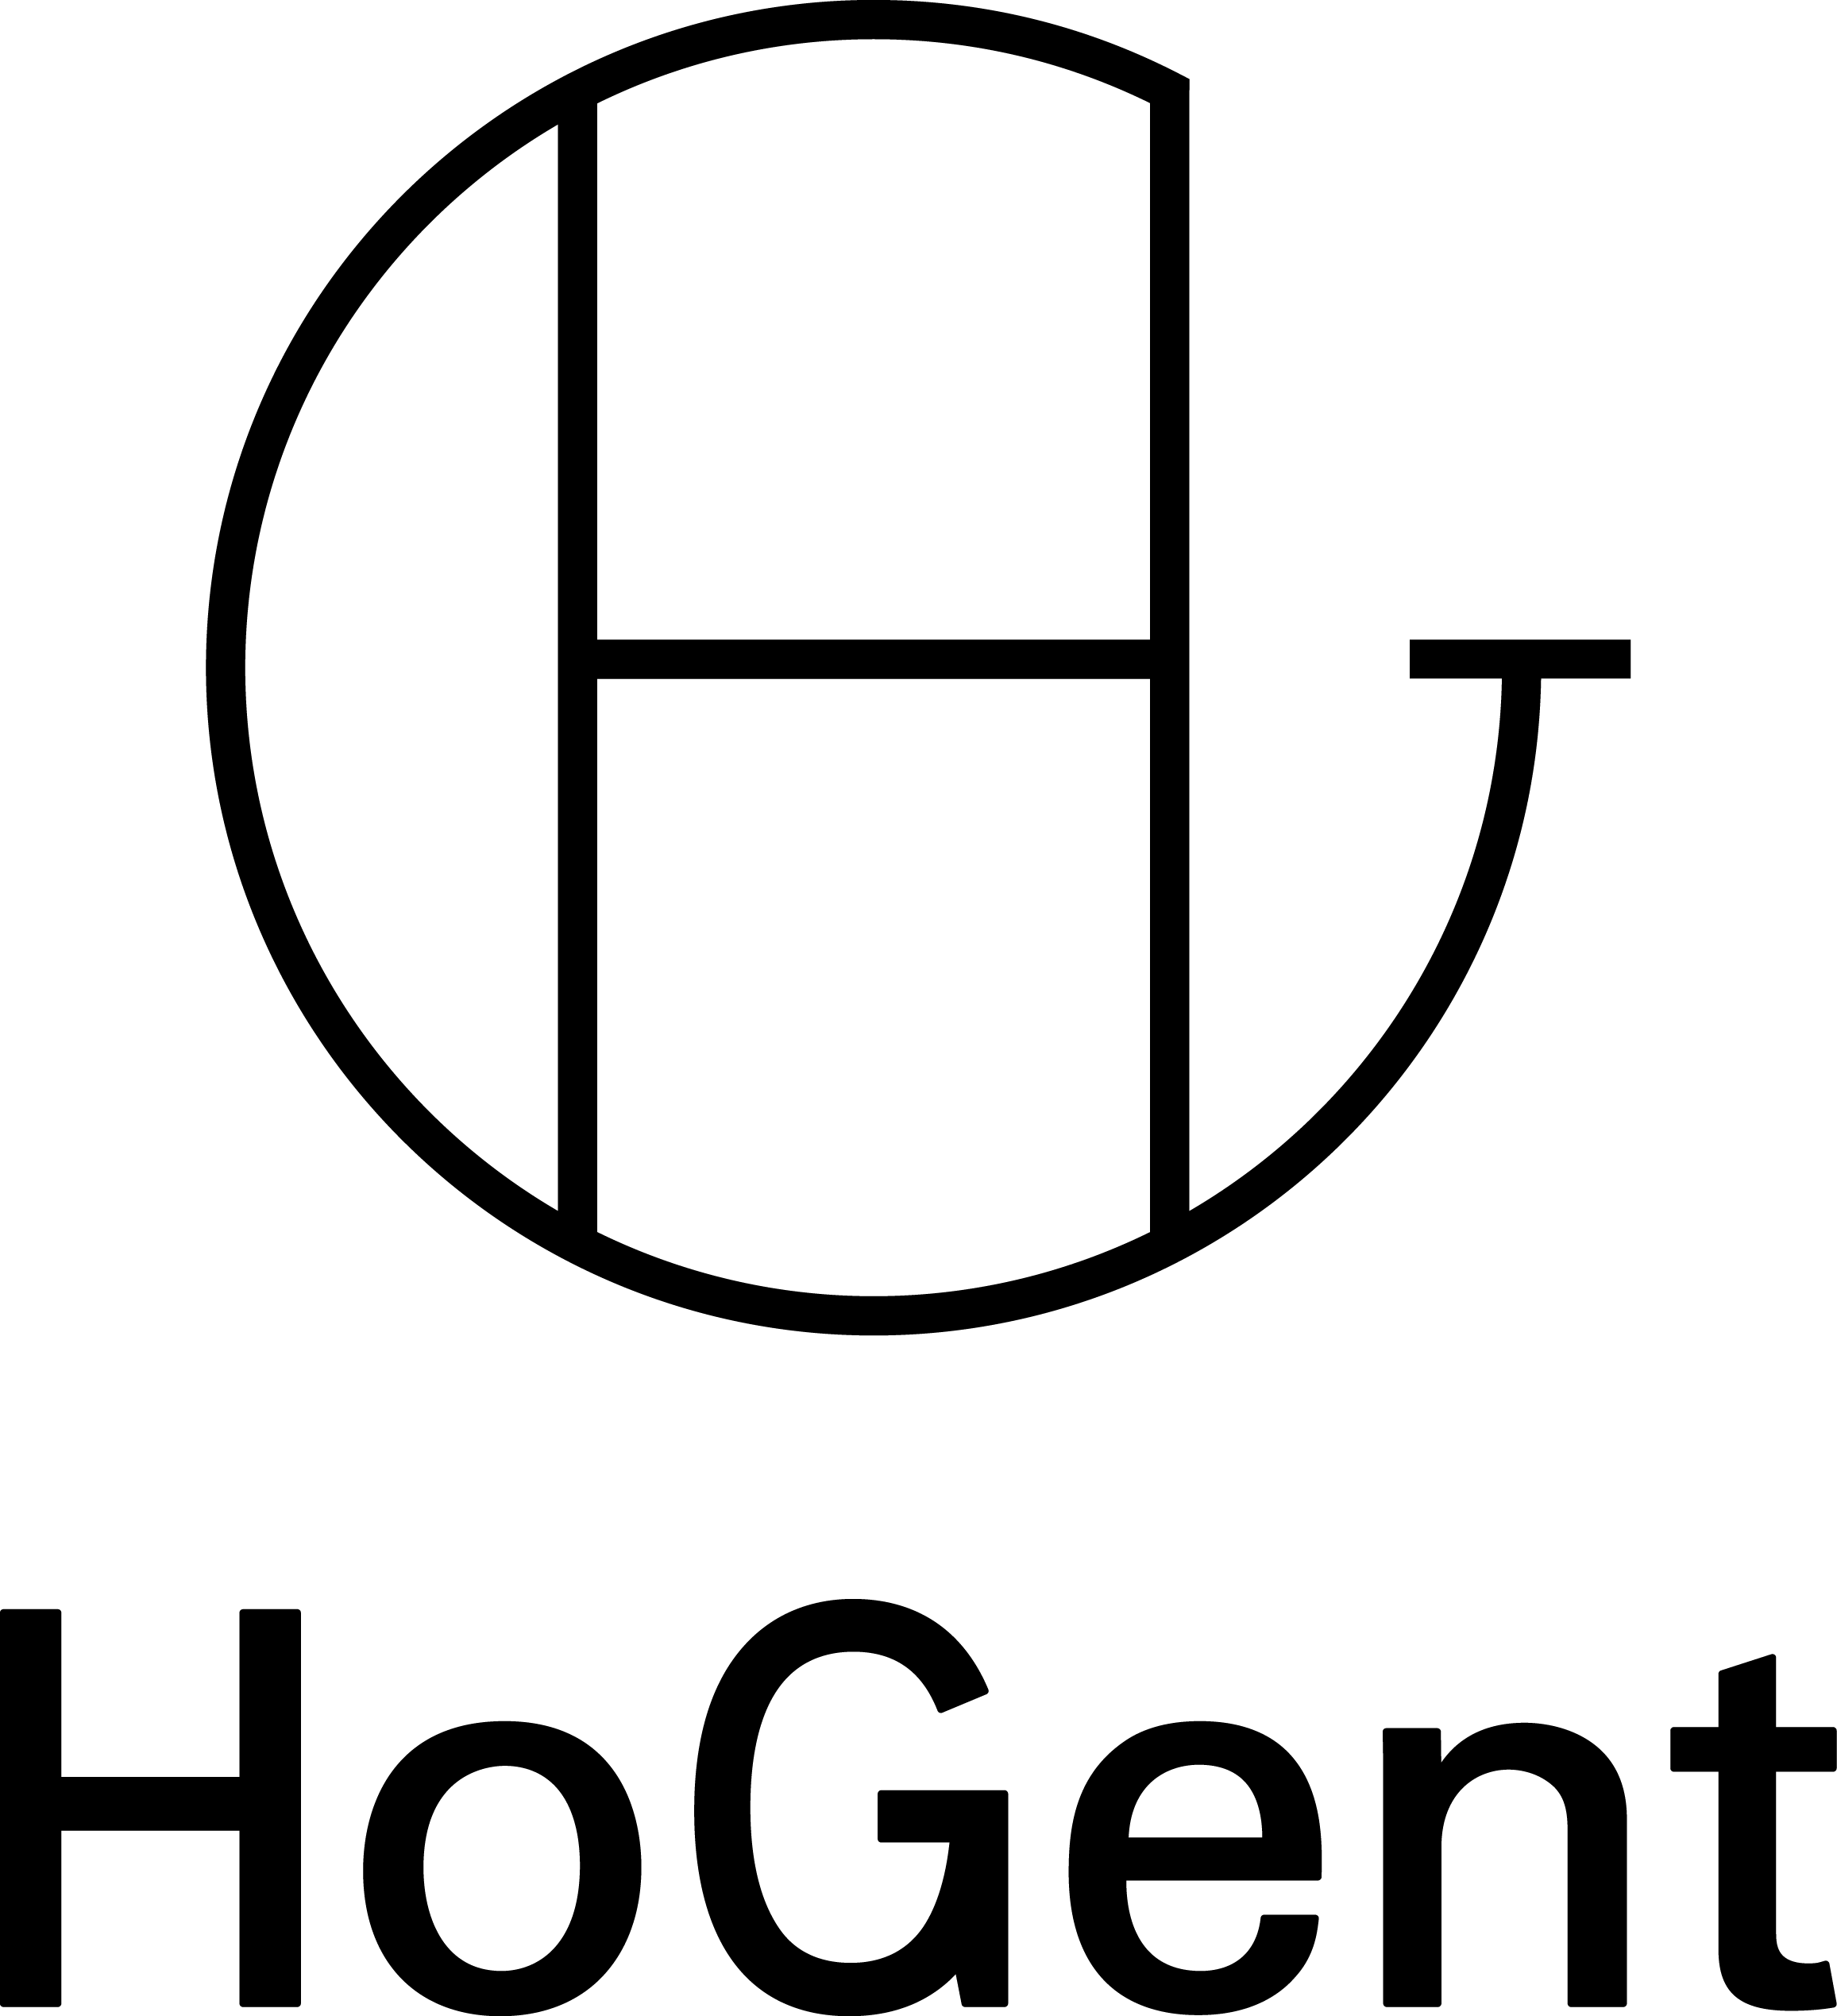
\includegraphics[width=2.5cm]{img/HG-beeldmerk-woordmerk}\\[.5cm]
    Faculteit Bedrijf en Organisatie\\[3cm]
    \titel
    \vfill
    \student\\[3.5cm]
    Scriptie voorgedragen tot het bekomen van de graad van\\professionele bachelor in de toegepaste informatica\\[2cm]
    Promotor:\\
    \promotor\\
    \ifdefempty{\copromotor}{\vspace{2.5cm}}{Co-promotor:\\\copromotor\\[2.5cm]}
    Instelling: \instelling\\[.5cm]
    Academiejaar: \academiejaar\\[.5cm]
    \ifcase \examenperiode \or Eerste \or Tweede \else Derde \fi examenperiode
    \endgroup

  \end{center}
  \restoregeometry
\end{titlepage}
  \emptypage
\begin{titlepage}
  \newgeometry{top=5.35cm,bottom=1.5cm,left=1.5cm,right=1.5cm}
  \begin{center}

    \begingroup
    \rmfamily
    \IfLanguageName{dutch}{Faculteit Bedrijf en Organisatie}{Faculty of Business and Information Management}\\[3cm]
    \titel
    \vfill
    \student\\[3.5cm]
    \IfLanguageName{dutch}{Scriptie voorgedragen tot het bekomen van de graad van\\professionele bachelor in de toegepaste informatica}{Thesis submitted in partial fulfilment of the requirements for the degree of\\professional bachelor of applied computer science}\\[2cm]
    Promotor:\\
    \promotor\\
    \ifdefempty{\copromotor}{\vspace{2.5cm}}{Co-promotor:\\\copromotor\\[2.5cm]}
    \IfLanguageName{dutch}{Instelling}{Institution}: \instelling\\[.5cm]
    \IfLanguageName{dutch}{Academiejaar}{Academic year}: \academiejaar\\[.5cm]
    \IfLanguageName{dutch}{%
    \ifcase \examenperiode \or Eerste \or Tweede \else Derde \fi examenperiode}{%
    \ifcase \examenperiode \or First \or Second \else Third \fi examination period}
    \endgroup

  \end{center}
  \restoregeometry
\end{titlepage}
}

%----------------------------------------------------------------------------------------
%	BIBLIOGRAPHY AND INDEX
%----------------------------------------------------------------------------------------

\usepackage[style=apa,backend=biber]{biblatex}
\usepackage{csquotes}
\DeclareLanguageMapping{dutch}{dutch-apa}
\addbibresource{bachproef-tin.bib} % BibTeX bibliography file
\defbibheading{bibempty}{}

\usepackage{calc} % For simpler calculation - used for spacing the index letter headings correctly
\usepackage{makeidx} % Required to make an index
\makeindex % Tells LaTeX to create the files required for indexing

%----------------------------------------------------------------------------------------
%	MAIN TABLE OF CONTENTS
%----------------------------------------------------------------------------------------

\usepackage{titletoc} % Required for manipulating the table of contents

\contentsmargin{0cm} % Removes the default margin

% Part text styling
\titlecontents{part}[0cm]
{\addvspace{20pt}\centering\large\bfseries}
{}
{}
{}

% Chapter text styling
\titlecontents{chapter}[1.25cm] % Indentation
{\addvspace{12pt}\large\sffamily\bfseries} % Spacing and font options for chapters
{\color{maincolor!60}\contentslabel[\Large\thecontentslabel]{1.25cm}\color{maincolor}} % Chapter number
{\color{maincolor}}
{\color{maincolor!60}\normalsize\;\titlerule*[.5pc]{.}\;\thecontentspage} % Page number

% Section text styling
\titlecontents{section}[1.25cm] % Indentation
{\addvspace{3pt}\sffamily\bfseries} % Spacing and font options for sections
{\contentslabel[\thecontentslabel]{1.25cm}} % Section number
{}
{\hfill\color{black}\thecontentspage} % Page number
[]

% Subsection text styling
\titlecontents{subsection}[1.25cm] % Indentation
{\addvspace{1pt}\sffamily\small} % Spacing and font options for subsections
{\contentslabel[\thecontentslabel]{1.25cm}} % Subsection number
{}
{\ \titlerule*[.5pc]{.}\;\thecontentspage} % Page number
[]

% List of figures
\titlecontents{figure}[0em]
{\addvspace{-5pt}\sffamily}
{\thecontentslabel\hspace*{1em}}
{}
{\ \titlerule*[.5pc]{.}\;\thecontentspage}
[]

% List of tables
\titlecontents{table}[0em]
{\addvspace{-5pt}\sffamily}
{\thecontentslabel\hspace*{1em}}
{}
{\ \titlerule*[.5pc]{.}\;\thecontentspage}
[]

%----------------------------------------------------------------------------------------
%	MINI TABLE OF CONTENTS IN PART HEADS
%----------------------------------------------------------------------------------------

% Chapter text styling
\titlecontents{lchapter}[0em] % Indenting
{\addvspace{15pt}\large\sffamily\bfseries} % Spacing and font options for chapters
{\color{maincolor}\contentslabel[\Large\thecontentslabel]{1.25cm}\color{maincolor}} % Chapter number
{}
{\color{maincolor}\normalsize\sffamily\bfseries\;\titlerule*[.5pc]{.}\;\thecontentspage} % Page number

% Section text styling
\titlecontents{lsection}[0em] % Indenting
{\sffamily\small} % Spacing and font options for sections
{\contentslabel[\thecontentslabel]{1.25cm}} % Section number
{}
{}

% Subsection text styling
\titlecontents{lsubsection}[.5em] % Indentation
{\normalfont\footnotesize\sffamily} % Font settings
{}
{}
{}

%----------------------------------------------------------------------------------------
%	PAGE HEADERS
%----------------------------------------------------------------------------------------

\usepackage{fancyhdr} % Required for header and footer configuration

\pagestyle{fancy}
\renewcommand{\chaptermark}[1]{\markboth{\sffamily\normalsize\bfseries\chaptername\ \thechapter.\ #1}{}} % Chapter text font settings
\renewcommand{\sectionmark}[1]{\markright{\sffamily\normalsize\thesection\hspace{5pt}#1}{}} % Section text font settings
\fancyhf{} \fancyhead[LE,RO]{\sffamily\normalsize\thepage} % Font setting for the page number in the header
\fancyhead[LO]{\rightmark} % Print the nearest section name on the left side of odd pages
\fancyhead[RE]{\leftmark} % Print the current chapter name on the right side of even pages
\renewcommand{\headrulewidth}{0.5pt} % Width of the rule under the header
\addtolength{\headheight}{2.5pt} % Increase the spacing around the header slightly
\renewcommand{\footrulewidth}{0pt} % Removes the rule in the footer
\fancypagestyle{plain}{\fancyhead{}\renewcommand{\headrulewidth}{0pt}} % Style for when a plain pagestyle is specified

% Removes the header from odd empty pages at the end of chapters
\makeatletter
\renewcommand{\cleardoublepage}{
\clearpage\ifodd\c@page\else
\hbox{}
\vspace*{\fill}
\thispagestyle{empty}
\newpage
\fi}

%----------------------------------------------------------------------------------------
%	THEOREM STYLES
%----------------------------------------------------------------------------------------

\usepackage{amsmath,amsfonts,amssymb,amsthm} % For math equations, theorems, symbols, etc

\newcommand{\intoo}[2]{\mathopen{]}#1\,;#2\mathclose{[}}
\newcommand{\ud}{\mathop{\mathrm{{}d}}\mathopen{}}
\newcommand{\intff}[2]{\mathopen{[}#1\,;#2\mathclose{]}}
\newtheorem{notation}{Notation}[chapter]

% Boxed/framed environments
\newtheoremstyle{maincolornumbox}% % Theorem style name
{0pt}% Space above
{0pt}% Space below
{\normalfont}% % Body font
{}% Indent amount
{\small\bf\sffamily\color{maincolor}}% % Theorem head font
{\;}% Punctuation after theorem head
{0.25em}% Space after theorem head
{\small\sffamily\color{maincolor}\thmname{#1}\nobreakspace\thmnumber{\@ifnotempty{#1}{}\@upn{#2}}% Theorem text (e.g. Theorem 2.1)
\thmnote{\nobreakspace\the\thm@notefont\sffamily\bfseries\color{black}---\nobreakspace#3.}} % Optional theorem note
\renewcommand{\qedsymbol}{$\blacksquare$}% Optional qed square

\newtheoremstyle{blacknumex}% Theorem style name
{5pt}% Space above
{5pt}% Space below
{\normalfont}% Body font
{} % Indent amount
{\small\bf\sffamily}% Theorem head font
{\;}% Punctuation after theorem head
{0.25em}% Space after theorem head
{\small\sffamily{\tiny\ensuremath{\blacksquare}}\nobreakspace\thmname{#1}\nobreakspace\thmnumber{\@ifnotempty{#1}{}\@upn{#2}}% Theorem text (e.g. Theorem 2.1)
\thmnote{\nobreakspace\the\thm@notefont\sffamily\bfseries---\nobreakspace#3.}}% Optional theorem note

\newtheoremstyle{blacknumbox} % Theorem style name
{0pt}% Space above
{0pt}% Space below
{\normalfont}% Body font
{}% Indent amount
{\small\bf\sffamily}% Theorem head font
{\;}% Punctuation after theorem head
{0.25em}% Space after theorem head
{\small\sffamily\thmname{#1}\nobreakspace\thmnumber{\@ifnotempty{#1}{}\@upn{#2}}% Theorem text (e.g. Theorem 2.1)
\thmnote{\nobreakspace\the\thm@notefont\sffamily\bfseries---\nobreakspace#3.}}% Optional theorem note

% Non-boxed/non-framed environments
\newtheoremstyle{maincolornum}% % Theorem style name
{5pt}% Space above
{5pt}% Space below
{\normalfont}% % Body font
{}% Indent amount
{\small\bf\sffamily\color{maincolor}}% % Theorem head font
{\;}% Punctuation after theorem head
{0.25em}% Space after theorem head
{\small\sffamily\color{maincolor}\thmname{#1}\nobreakspace\thmnumber{\@ifnotempty{#1}{}\@upn{#2}}% Theorem text (e.g. Theorem 2.1)
\thmnote{\nobreakspace\the\thm@notefont\sffamily\bfseries\color{black}---\nobreakspace#3.}} % Optional theorem note
\renewcommand{\qedsymbol}{$\blacksquare$}% Optional qed square
\makeatother

% Defines the theorem text style for each type of theorem to one of the three styles above
\newcounter{dummy}
\numberwithin{dummy}{section}
\theoremstyle{maincolornumbox}
\newtheorem{theoremeT}[dummy]{Theorem}
\newtheorem{problem}{Problem}[chapter]
\newtheorem{exerciseT}{Exercise}[chapter]
\theoremstyle{blacknumex}
\newtheorem{exampleT}{Example}[chapter]
\theoremstyle{blacknumbox}
\newtheorem{vocabulary}{Vocabulary}[chapter]
\newtheorem{definitionT}{Definition}[section]
\newtheorem{corollaryT}[dummy]{Corollary}
\theoremstyle{maincolornum}
\newtheorem{proposition}[dummy]{Proposition}

%----------------------------------------------------------------------------------------
%	DEFINITION OF COLORED BOXES
%----------------------------------------------------------------------------------------

\RequirePackage[framemethod=default]{mdframed} % Required for creating the theorem, definition, exercise and corollary boxes

% Theorem box
\newmdenv[skipabove=7pt,
skipbelow=7pt,
backgroundcolor=black!5,
linecolor=maincolor,
innerleftmargin=5pt,
innerrightmargin=5pt,
innertopmargin=5pt,
leftmargin=0cm,
rightmargin=0cm,
innerbottommargin=5pt]{tBox}

% Exercise box
\newmdenv[skipabove=7pt,
skipbelow=7pt,
rightline=false,
leftline=true,
topline=false,
bottomline=false,
backgroundcolor=maincolor!10,
linecolor=maincolor,
innerleftmargin=5pt,
innerrightmargin=5pt,
innertopmargin=5pt,
innerbottommargin=5pt,
leftmargin=0cm,
rightmargin=0cm,
linewidth=4pt]{eBox}

% Definition box
\newmdenv[skipabove=7pt,
skipbelow=7pt,
rightline=false,
leftline=true,
topline=false,
bottomline=false,
linecolor=maincolor,
innerleftmargin=5pt,
innerrightmargin=5pt,
innertopmargin=0pt,
leftmargin=0cm,
rightmargin=0cm,
linewidth=4pt,
innerbottommargin=0pt]{dBox}

% Corollary box
\newmdenv[skipabove=7pt,
skipbelow=7pt,
rightline=false,
leftline=true,
topline=false,
bottomline=false,
linecolor=gray,
backgroundcolor=black!5,
innerleftmargin=5pt,
innerrightmargin=5pt,
innertopmargin=5pt,
leftmargin=0cm,
rightmargin=0cm,
linewidth=4pt,
innerbottommargin=5pt]{cBox}

% Creates an environment for each type of theorem and assigns it a theorem text style from the "Theorem Styles" section above and a colored box from above
\newenvironment{theorem}{\begin{tBox}\begin{theoremeT}}{\end{theoremeT}\end{tBox}}
\newenvironment{exercise}{\begin{eBox}\begin{exerciseT}}{\hfill{\color{maincolor}\tiny\ensuremath{\blacksquare}}\end{exerciseT}\end{eBox}}
\newenvironment{definition}{\begin{dBox}\begin{definitionT}}{\end{definitionT}\end{dBox}}
\newenvironment{example}{\begin{exampleT}}{\hfill{\tiny\ensuremath{\blacksquare}}\end{exampleT}}
\newenvironment{corollary}{\begin{cBox}\begin{corollaryT}}{\end{corollaryT}\end{cBox}}

%----------------------------------------------------------------------------------------
%	REMARK ENVIRONMENT
%----------------------------------------------------------------------------------------

\newenvironment{remark}{\par\vspace{10pt}\small % Vertical white space above the remark and smaller font size
\begin{list}{}{
\leftmargin=35pt % Indentation on the left
\rightmargin=25pt}\item\ignorespaces % Indentation on the right
\makebox[-2.5pt]{\begin{tikzpicture}[overlay]
\node[draw=maincolor!60,line width=1pt,circle,fill=maincolor!25,font=\sffamily\bfseries,inner sep=2pt,outer sep=0pt] at (-15pt,0pt){\textcolor{maincolor}{R}};\end{tikzpicture}} % Orange R in a circle
\advance\baselineskip -1pt}{\end{list}\vskip5pt} % Tighter line spacing and white space after remark

%----------------------------------------------------------------------------------------
%	SECTION NUMBERING IN THE MARGIN
%----------------------------------------------------------------------------------------

\makeatletter
\renewcommand{\@seccntformat}[1]{\llap{\textcolor{maincolor}{\csname the#1\endcsname}\hspace{1em}}}
\renewcommand{\section}{\@startsection{section}{1}{\z@}
{-4ex \@plus -1ex \@minus -.4ex}
{1ex \@plus.2ex }
{\normalfont\large\sffamily\bfseries}}
\renewcommand{\subsection}{\@startsection {subsection}{2}{\z@}
{-3ex \@plus -0.1ex \@minus -.4ex}
{0.5ex \@plus.2ex }
{\normalfont\sffamily\bfseries}}
\renewcommand{\subsubsection}{\@startsection {subsubsection}{3}{\z@}
{-2ex \@plus -0.1ex \@minus -.2ex}
{.2ex \@plus.2ex }
{\normalfont\small\sffamily\bfseries}}
\renewcommand\paragraph{\@startsection{paragraph}{4}{\z@}
{-2ex \@plus-.2ex \@minus .2ex}
{.1ex}
{\normalfont\small\sffamily\bfseries}}

%----------------------------------------------------------------------------------------
%	PART HEADINGS
%----------------------------------------------------------------------------------------

% numbered part in the table of contents
\newcommand{\@mypartnumtocformat}[2]{%
\setlength\fboxsep{0pt}%
\noindent\colorbox{maincolor!20}{\strut\parbox[c][.7cm]{\ecart}{\color{maincolor!70}\Large\sffamily\bfseries\centering#1}}\hskip\esp\colorbox{maincolor!40}{\strut\parbox[c][.7cm]{\linewidth-\ecart-\esp}{\Large\sffamily\centering#2}}}%
%%%%%%%%%%%%%%%%%%%%%%%%%%%%%%%%%%
% unnumbered part in the table of contents
\newcommand{\@myparttocformat}[1]{%
\setlength\fboxsep{0pt}%
\noindent\colorbox{maincolor!40}{\strut\parbox[c][.7cm]{\linewidth}{\Large\sffamily\centering#1}}}%
%%%%%%%%%%%%%%%%%%%%%%%%%%%%%%%%%%
\newlength\esp
\setlength\esp{4pt}
\newlength\ecart
\setlength\ecart{1.2cm-\esp}
\newcommand{\thepartimage}{}%
\newcommand{\partimage}[1]{\renewcommand{\thepartimage}{#1}}%
\def\@part[#1]#2{%
\ifnum \c@secnumdepth >-2\relax%
\refstepcounter{part}%
\addcontentsline{toc}{part}{\texorpdfstring{\protect\@mypartnumtocformat{\thepart}{#1}}{\partname~\thepart\ ---\ #1}}
\else%
\addcontentsline{toc}{part}{\texorpdfstring{\protect\@myparttocformat{#1}}{#1}}%
\fi%
\startcontents%
\markboth{}{}%
{\thispagestyle{empty}%
\begin{tikzpicture}[remember picture,overlay]%
\node at (current page.north west){\begin{tikzpicture}[remember picture,overlay]%
\fill[maincolor!20](0cm,0cm) rectangle (\paperwidth,-\paperheight);
\node[anchor=north] at (4cm,-3.25cm){\color{maincolor!40}\fontsize{220}{100}\sffamily\bfseries\@Roman\c@part};
\node[anchor=south east] at (\paperwidth-1cm,-\paperheight+1cm){\parbox[t][][t]{8.5cm}{
\printcontents{l}{0}{\setcounter{tocdepth}{1}}%
}};
\node[anchor=north east] at (\paperwidth-1.5cm,-3.25cm){\parbox[t][][t]{15cm}{\strut\raggedleft\color{white}\fontsize{30}{30}\sffamily\bfseries#2}};
\end{tikzpicture}};
\end{tikzpicture}}%
\@endpart}
\def\@spart#1{%
\startcontents%
\phantomsection
{\thispagestyle{empty}%
\begin{tikzpicture}[remember picture,overlay]%
\node at (current page.north west){\begin{tikzpicture}[remember picture,overlay]%
\fill[maincolor!20](0cm,0cm) rectangle (\paperwidth,-\paperheight);
\node[anchor=north east] at (\paperwidth-1.5cm,-3.25cm){\parbox[t][][t]{15cm}{\strut\raggedleft\color{white}\fontsize{30}{30}\sffamily\bfseries#1}};
\end{tikzpicture}};
\end{tikzpicture}}
\addcontentsline{toc}{part}{\texorpdfstring{%
\setlength\fboxsep{0pt}%
\noindent\protect\colorbox{maincolor!40}{\strut\protect\parbox[c][.7cm]{\linewidth}{\Large\sffamily\protect\centering #1\quad\mbox{}}}}{#1}}%
\@endpart}
\def\@endpart{\vfil\newpage
\if@twoside
\if@openright
\null
\thispagestyle{empty}%
\newpage
\fi
\fi
\if@tempswa
\twocolumn
\fi}

%----------------------------------------------------------------------------------------
%	CHAPTER HEADINGS
%----------------------------------------------------------------------------------------

% A switch to conditionally include a picture, implemented by  Christian Hupfer
\newif\ifusechapterimage
\usechapterimagetrue
\newcommand{\thechapterimage}{}%
\newcommand{\chapterimage}[1]{\ifusechapterimage\renewcommand{\thechapterimage}{#1}\fi}%
\def\@makechapterhead#1{%
{\parindent \z@ \raggedright \normalfont
\ifnum \c@secnumdepth >\m@ne
\if@mainmatter
\begin{tikzpicture}[remember picture,overlay]
\node at (current page.north west)
{\begin{tikzpicture}[remember picture,overlay]
\node[anchor=north west,inner sep=0pt] at (0,0) {\ifusechapterimage\includegraphics[width=\paperwidth]{\thechapterimage}\fi};
\draw[anchor=west] (\Gm@lmargin,-9cm) node [line width=2pt,rounded corners=15pt,draw=maincolor,fill=white,fill opacity=0.5,inner sep=15pt]{\strut\makebox[22cm]{}};
\draw[anchor=west] (\Gm@lmargin+.3cm,-9cm) node {\huge\sffamily\bfseries\color{black}\thechapter. #1\strut};
\end{tikzpicture}};
\end{tikzpicture}
\else
\begin{tikzpicture}[remember picture,overlay]
\node at (current page.north west)
{\begin{tikzpicture}[remember picture,overlay]
\node[anchor=north west,inner sep=0pt] at (0,0) {\ifusechapterimage\includegraphics[width=\paperwidth]{\thechapterimage}\fi};
\draw[anchor=west] (\Gm@lmargin,-9cm) node [line width=2pt,rounded corners=15pt,draw=maincolor,fill=white,fill opacity=0.5,inner sep=15pt]{\strut\makebox[22cm]{}};
\draw[anchor=west] (\Gm@lmargin+.3cm,-9cm) node {\huge\sffamily\bfseries\color{black}#1\strut};
\end{tikzpicture}};
\end{tikzpicture}
\fi\fi\par\vspace*{270\p@}}}

%-------------------------------------------

\def\@makeschapterhead#1{%
\begin{tikzpicture}[remember picture,overlay]
\node at (current page.north west)
{\begin{tikzpicture}[remember picture,overlay]
\node[anchor=north west,inner sep=0pt] at (0,0) {\ifusechapterimage\includegraphics[width=\paperwidth]{\thechapterimage}\fi};
\draw[anchor=west] (\Gm@lmargin,-9cm) node [line width=2pt,rounded corners=15pt,draw=maincolor,fill=white,fill opacity=0.5,inner sep=15pt]{\strut\makebox[22cm]{}};
\draw[anchor=west] (\Gm@lmargin+.3cm,-9cm) node {\huge\sffamily\bfseries\color{black}#1\strut};
\end{tikzpicture}};
\end{tikzpicture}
\par\vspace*{270\p@}}
\makeatother

%----------------------------------------------------------------------------------------
%	HYPERLINKS IN THE DOCUMENTS
%----------------------------------------------------------------------------------------

\usepackage{hyperref}
\hypersetup{hidelinks,backref=true,pagebackref=true,hyperindex=true,colorlinks=false,breaklinks=true,urlcolor= maincolor,bookmarks=true,bookmarksopen=false,pdftitle={Title},pdfauthor={Author}}
\usepackage{bookmark}
\bookmarksetup{
open,
numbered,
addtohook={%
\ifnum\bookmarkget{level}=0 % chapter
\bookmarksetup{bold}%
\fi
\ifnum\bookmarkget{level}=-1 % part
\bookmarksetup{color=maincolor,bold}%
\fi
}
}

%----------------------------------------------------------------------------------------
%	Java source code
%----------------------------------------------------------------------------------------

% Commando voor invoegen Java-broncodebestanden (dank aan Niels Corneille)
% Gebruik:
%   \codefragment{source/MijnKlasse.java}{Uitleg bij de code}
%
% Je kan dit aanpassen aan de taal die je zelf het meeste gebruikt in je
% bachelorproef.
\newcommand{\codefragment}[2]{ \lstset{%
  language=java,
  breaklines=true,
  float=th,
  caption={#2},
  basicstyle=\scriptsize,
  frame=single,
  extendedchars=\true
}
\lstinputlisting{#1}}

% Leeg blad
\newcommand{\emptypage}{%
\newpage
\thispagestyle{empty}
\mbox{}
\newpage
}


%%---------- Documenteigenschappen --------------------------------------------
%% TODO: Vul dit aan met je eigen info:

% Je eigen naam
\newcommand{\student}{Ruben Standaert}

% De naam van je promotor (lector van de opleiding)
\newcommand{\promotor}{Sabine De Vreese}

% De naam van je co-promotor. Als je promotor ook je opdrachtgever is en je
% dus ook inhoudelijk begeleidt (en enkel dan!), mag je dit leeg laten.
\newcommand{\copromotor}{Ken Vanderbeken}

% Indien je bachelorproef in opdracht van/in samenwerking met een bedrijf of
% externe organisatie geschreven is, geef je hier de naam. Zoniet laat je dit
% zoals het is.
\newcommand{\instelling}{Insites Consulting}

% De titel van het rapport/bachelorproef
\newcommand{\titel}{Data-analyse met Elasticsearch}

% Datum van indienen (gebruik telkens de deadline, ook al geef je eerder af)
\newcommand{\datum}{28 mei 2018}

% Academiejaar
\newcommand{\academiejaar}{2017-2018}

% Examenperiode
%  - 1e semester = 1e examenperiode => 1
%  - 2e semester = 2e examenperiode => 2
%  - tweede zit  = 3e examenperiode => 3
\newcommand{\examenperiode}{2}

%%=============================================================================
%% Inhoud document
%%=============================================================================

\begin{document}

%---------- Taalselectie ------------------------------------------------------
%% Als je je bachelorproef in het Engels schrijft, haal dan onderstaande regel
%% uit commentaar. Let op: de tekst op de voorkaft blijft in het Nederlands, en
%% dat is ook de bedoeling!
%\selectlanguage{english}

%---------- Titelblad ---------------------------------------------------------
\inserttitlepage

%---------- Samenvatting, voorwoord -------------------------------------------
\usechapterimagefalse
%%=============================================================================
%% Samenvatting
%%=============================================================================

%% TODO: De "abstract" of samenvatting is een kernachtige (~ 1 blz. voor een
%% thesis) synthese van het document.
%%
%% Deze aspecten moeten zeker aan bod komen:
%% - Context: waarom is dit werk belangrijk?
%% - Nood: waarom moest dit onderzocht worden?
%% - Taak: wat heb je precies gedaan?
%% - Object: wat staat in dit document geschreven?
%% - Resultaat: wat was het resultaat?
%% - Conclusie: wat is/zijn de belangrijkste conclusie(s)?
%% - Perspectief: blijven er nog vragen open die in de toekomst nog kunnen
%%    onderzocht worden? Wat is een mogelijk vervolg voor jouw onderzoek?
%%
%% LET OP! Een samenvatting is GEEN voorwoord!

%%---------- Nederlandse samenvatting -----------------------------------------
%%
%% TODO: Als je je bachelorproef in het Engels schrijft, moet je eerst een
%% Nederlandse samenvatting invoegen. Haal daarvoor onderstaande code uit
%% commentaar.
%% Wie zijn bachelorproef in het Nederlands schrijft, kan dit negeren en heel
%% deze sectie verwijderen.

\IfLanguageName{english}{%
\selectlanguage{dutch}
\chapter*{Samenvatting}
\lipsum[1-4]
\selectlanguage{english}
}{}

%%---------- Samenvatting -----------------------------------------------------
%%
%% De samenvatting in de hoofdtaal van het document

\chapter*{\IfLanguageName{dutch}{Samenvatting}{Abstract}}


%%=============================================================================
%% Voorwoord
%%=============================================================================

\chapter{Voorwoord}
\label{ch:voorwoord}

%% TODO:
%% Het voorwoord is het enige deel van de bachelorproef waar je vanuit je
%% eigen standpunt (``ik-vorm'') mag schrijven. Je kan hier bv. motiveren
%% waarom jij het onderwerp wil bespreken.
%% Vergeet ook niet te bedanken wie je geholpen/gesteund/... heeft

Het onderzoek in deze bachelorproef werd uitgevoerd in functie van het behalen van mijn diploma Toegepaste Informatica aan de hogeschool HoGent. Het idee voor deze bachelorproef komt van Sabine De Vreese die lector is aan de hogeschool HoGent. Ik kwam bij haar met de vraag of ze enkele interessante onderwerpen kende waarbij data centraal staat. Één van de onderwerpen de ze mij aanreikte was Elasticsearch. Nooit eerder had ik van Elasticsearch gehoord. Na wat opzoekingswerk werd snel duidelijk dat Elasticsearch door veel grote bedrijven en voor een verscheidenheid aan use cases gebruikt wordt. Het is een zoekmachine die samen met haar community nog steeds aan het groeien is maar ook een aantal alternatieven heeft. Om een breder inzicht te kunnen geven in wanneer men Elasticsearch best verkiest deed ik een onderzoek naar de voor-en nadelen van de zoekmachine. In dat onderzoek mikte ik vooral op data-analyse met Elasticsearch. Bij deze wil ik Sabine De Vreese graag bedanken voor het aanreiken van dit interessant onderwerp. Gedurende het onderzoek heeft Sabine De Vreese ook de rol van promotor op zich genomen. Ze heeft me wekelijks begeleid en bijgestuurd waar nodig. Ook daarvoor wil ik haar graag bedanken. Als laatste wil ik mijn co-promotor Ken Vanderbeken bedanken. Hij bezorgde mij een dataset die ik nodig had om een project in Elasticsearch op te zetten. Naast de dataset kreeg ik ook een aantal vragen die ik in dat project kon oplossen.



%---------- Inhoudstafel ------------------------------------------------------
\pagestyle{empty} % No headers
\tableofcontents % Print the table of contents itself
\cleardoublepage % Forces the first chapter to start on an odd page so it's on the right
\pagestyle{fancy} % Print headers again

%---------- Lijst afkortingen, termen -----------------------------------------
%% Als je een lijst van afkortingen of termen wil toevoegen, dan hoort die
%% hier thuis. Gebruik bijvoorbeeld de ``glossaries'' package.

%%---------- Kern -------------------------------------------------------------

%%=============================================================================
%% Inleiding
%%=============================================================================

\chapter{Inleiding}
\label{ch:inleiding}

\section{Stand van zaken}
\label{sec:stand-van-zaken}

Elasticsearch is een zoekmachine die in Java geschreven is. De zoekmachine werd boven de Java library Apache Lucene gebouwd. Alle commando's worden verzonden door middel van HTTP requests naar de Elasticsearch REST API. Die API is gebaseerd op JSON. Dat wil zeggen dat de mogelijkheid bestaat om JSON mee te geven aan de HTTP requests. Ook de resultaten worden in JSON teruggegeven. Elasticsearch is niet enkel een zoekmachine maar wordt ook gebruikt voor data-analyses en om aan logging te doen. 

Shay Bannon ontwierp Elasticsearch als een gedistribueerd systeem. Een gedistribueerd systeem brengt zowel voordelen als nadelen met zich mee. Volgens \textcite{Brasetvik2013} focussen verschillende systemen op verschillende sterktes, afhankelijk van welke eigenschappen belangrijker zijn voor het systeem. Daarbij wordt gezegd dat Elasticsearch focust op snelheid. Het streeft naar real-time search. Om dat de kunnen bereiken in een gedistribueerd systeem worden een aantal zaken aan de kant geschoven of vereenvoudigd. Een voorbeeld hiervan is concurrency control. Die wordt gedaan aan de hand van versienummers van de documents. Dit is wat we noemen een optimistische aanpak. Deze manier van werken zorgt ervoor dat het systeem zich niet moet bezighouden met locks. Met locks bedoelt men dat, wanneer een transactie aan het schrijven is, niemand anders naar dezelfde tabel kan schrijven totdat de transactie is voltooid. Er wordt namelijk een slot geplaatst op te tabel zolang deze bezet is. Het is duidelijk dat het werken met versienummers minder complexiteit met zich meebrengt dan het werken met locks. Daarom is de optimistische concurrency control performanter. Dat is echter enkel zo in een systeem waar de data niet veel aangepast wordt. Wanneer de data wel frequent aangepast wordt kan het zijn dat de optimistische aanpak juist minder performant wordt dan de pessimistische aanpak met de locks. Wanneer het systeem bij de validatie op het versienummer merkt dat de data veranderd is, moet de gehele transactie namelijk opnieuw gestart worden. De bedoeling van de optimistische aanpak is dat men over real-time search kan spreken. Wanneer men in een omgeving werkt met data die frequent verandert moet men rekening houden dat men de eigenschappen van real-time search kan verliezen. Een tweede manier om aan snelheid te winnen in een gedistribueerd systeem is caching. Elasticsearch doet vaak aan caching om niet telkens opnieuw alle data te moeten opvragen. Dat heeft een negatief effect op het geheugen dat het systeem nodig heeft maar ook een zeer positief effect op de uitvoeringstijd.

Het CAP theorema stelt dat het onmogelijk is voor een gedistribueerd systeem om gelijktijdig consistent (Consistent), beschikbaar (Available) en partitie tolerant (Partition tolerant) te zijn. Het stelt dat een gedistribueerd systeem tegelijk aan maximaal twee van de voornoemde eigenschappen kan voldoen. Consistent betekent dat alle nodes in de cluster dezelfde data zien op hetzelfde moment. Daarbij is het belangrijk dat deze data de meest recente data is. Men kan spreken over een beschikbaar systeem wanneer alle nodes een reponse kunnen geven voor alle requests. Wanneer een node geen response kan geven op een request wordt er niet aan de criteria voldaan om over een beschikbaar systeem te kunnen spreken. De laatste voorwaarde in het CAP theorema, partitie tolerant, houdt in dat het systeem correct blijft functioneren bij het uitvallen van een node in het netwerk. Volgens \textcite{Brasetvik2013} is het bij Elasticsearch over het algemeen zo dat het systeem consistent en partitie tolerant is. Dat noemt men een CP-systeem. Hierbij is het niet onbelangrijk om te vermelden dat er een zwakke definitie voor consistentie gebruikt wordt. Wat er precies gegarandeerd wordt is namelijk document consistentie waarbij er sprake is van consistentie binnen een document. Wanneer men Elasticsearch enkel gebruikt om data uit te lezen bereikt men een systeem dat beschikbaar en partitie tolerant is. Dat noemt men een AP-systeem.

\textcite{Glauner2012} schrijft dat één van de belangrijkste sterktes van de zoekmachine is dat het gebruik maakt van een schema-less data model. Hierdoor kan elk JSON document aan Elasticsearch toegevoegd worden. Dat zorgt voor veel flexibiliteit en minder configuratiewerk voor de gebruikers. \textcite{Brasetvik2013} gebruikt liever de term schema flexible. Er is namelijk wel een schema, alleen moet dat niet verplicht meegegeven worden. Het is perfect mogelijk dat een document enkele fields ontbreekt. Wanneer dat field gebruikt wordt in een zoekopdracht wordt het document niet meegenomen in de resultaten. De zoekmachine is zeer sterk in het herkennen van eenvoudige datatypes zoals nummers, booleans en timestamps. Daardoor kan er een impliciet schema gegenereerd worden zonder expliciet te moeten meegeven wat de datatypes zijn. De mogelijkheid om een schema mee te geven bestaat echter wel. Een reden om zelf een schema mee te geven is om de data op punt te stellen en zo de zoeksnelheden te doen laten stijgen.

\subsection{Apache Lucene}

Om een goed inzicht te krijgen in de architectuur en werking van Elasticsearch keert men beter eerst terug naar de basis. Die basis is Apache Lucene. Elasticsearch is namelijk een laag die bovenop Apache Lucene werd gebouwd. Wanneer de architectuur van Elasticsearch besproken wordt in sectie \ref{architectuur} zal het duidelijk worden waar Apache Lucene zich bevindt in die architectuur.

Apache Lucene is een gratis en open source full-text search Java library. Lucene werd origineel in Java geschreven maar werd later ook beschikbaar gemaakt in verscheidene programmeertalen zoals: C++, C\#, Delphi, Perl, PHP, Python, en Ruby \autocite{Whissel2009}. Deze library kan in een project geladen worden waardoor de functies kunnen aangeroepen worden.

\subsubsection{Features}

Er zijn een aantal features beschikbaar zoals: field searches, boolean operators, range searches en wildcard searches. Bij field searches kan de gebruiker specifiëren waar in het document er precies moet gezocht worden. Wanneer men een lijst van boeken van een specifieke auteur wil opvragen zal het systeem enkel naar het auteur veld kijken. Wanneer de naam van de auteur in bijvoorbeeld de titel voorkomt zal het boek niet in de zoekresultaten terechtkomen. De boolean operators laten de gebruiker toe om voorwaarden te combineren. Dat kan gerealiseerd worden door bijvoorbeeld de AND, OR en NOT operators te gebruiken. De AND en OR operators worden telkens tussen twee voorwaarden geplaatst om het resultaat te beïnvloeden. Ze geven aan dat er respectievelijk aan beide of minstens één voorwaarde moet voldaan worden vooraleer het document in de zoekresultaten terecht komt. De NOT operator hoort bij één voorwaarde en draait het resultaat van de voorwaarde om. Er kunnen haakjes rond de voorwaarden geplaatst worden om die te gaan groeperen.

Range searches laten toe om te gaan zoeken naar documents waarvan een bepaalde waarde tussen twee grenzen ligt. Zo kan men bijvoorbeeld zoeken naar alle personen met een leeftijd tussen 18 en 25 jaar. Bij wildcard searches wordt het mogelijk gemaakt om speciale symbolen mee te geven ter vervanging van tekst. Het ‘*’ symbool kan vervangen worden door meerdere karakters terwijl het ‘?’ symbool slechts door één karakter kan vervangen worden. 

Deze features bieden een zekere basisfunctionaliteit maar zijn niet altijd voldoende om aan elke use case te voldoen. Volgens \textcite{Whissel2009} zijn er daarom verschillende projecten, waaronder Elasticsearch, die de bestaande features van Lucene uitbreiden of nieuwe features toevoegen. Ze gebruiken dus Apache Lucene als basis.

\subsubsection{Architectuur}

Een document stelt een record voor en bestaat uit een aantal fields waarbij zo’n field uit een aantal terms bestaat. Een term is een eenvoudig stukje tekst. Lucene slaat alle informatie van de documents, die het nodig heeft om te zoeken, op in bestanden die men indices noemt. Die indices worden onderverdeeld in segments. Bij een zoekopdracht zullen de segment individueel doorzocht worden waarna de resultaten gecombineerd worden. De inhoud van een segment kan nooit veranderen. Wanneer er een document verwijderd wordt zal deze nog steeds terug te vinden zijn in het segment waar het oorspronkelijk opgeslaan werd. Lucene houdt bij welke documents er verwijderd zijn. Dat gebeurt aan de hand van een bitmap. In een zoekopdracht worden de documents, waarvan in de bitmap terug te vinden is dat die verwijderd zijn, uit de resultaten gefilterd. Het is echter niet interessant om grote aantallen verwijderde documents te bewaren in het geheugen. Ook zijn er veel situaties waarbij documents niet enkel verwijderd, maar ook aangepast of toegevoegd worden. Daarom wordt er regelmatig een nieuw segment aangemaakt die de recentere data bevat. Standaard gebeurt dit elke second. Om een overhead aan segments tegen te gaan worden segments samengevoegd tot één segment waar mogelijk. Bij die samenvoeging worden documents die als verwijderd gemarkeerd staan in de bitmap niet meegenomen. Door dit fenomeen is het mogelijk dat een index kleiner wordt wanneer men er een document aan toevoegd. Het kan zijn dat het toevoegen van een document een reactie van het systeem uitlokt om segments te gaan samenvoegen tot één segment. \autocite{Brasetvik2017}

Tot nu toe werd er enkel gesproken over het opslaan van documents. Een document wordt echter niet zomaar opgeslaan. In plaats van volledige documents op te slaan wordt er informatie over de terms opgeslaan. Informatie die bijgehouden wordt is onder andere: het rangnummer van de term in het bijhorende field, de lengte van de term en de positie van de term in het field. In plaats van per document bij te houden welke terms erbij horen, wordt er een lijst gemaakt van welke documents bij welke term horen. Dit heet reverted indexing. Zo kan het systeem een term opzoeken en teruggeven welke documents bij de term horen. \autocite{Whissel2009}

De reverted index is niet zo'n interessant gegeven wanneer men een term van een vooraf bepaald document wil opzoeken. Daarom wordt er per document ook een stored field opgeslaan. Een stored field is een key-value store die de data van het document voorstelt. Op die manier moet de reverted index niet volledig doorlopen worden maar kan men rechtstreeks data van het specifieke document opvragen.

\subsection{Elasticsearch architectuur}
\label{architectuur}


Om dit onderzoek beter te begrijpen worden de belangrijkste termen uit het domein van Elasticsearch eerst kort besproken. In het boek van \textcite{Dixit2016} leert men hoe de achterliggende structuur van Elasticsearch in elkaar zit. Elasticsearch bestaat uit een cluster. De eerste cluster heeft standaard Elasticsearch als naam. Alle clusters samen stellen de data voor. In figuur \ref{fig:ESArchitecture} van \textcite{Babaev2013} is te zien hoe zo'n cluster in elkaar zit. Een node is een instantie van Elasticsearch. Bij de creatie krijgt een node standaard een UUID en komt bij de Elasticsearch cluster tenzij anders gedefinieerd. In de nodes zitten de indices. Een index is een verzameling van documents met gelijkaardige karakteristieken. Hier slaat Elasticsearch data in op. Een index kan zeer groot worden. Het kan gebeuren dat de index te groot wordt om op de schijf van een node op te slaan. Daarom bestaat een index uit meerdere shards en replicas. Deze worden door Elasticsearch voorzien om een index op te delen in stukken. Een shard in Elasticsearch stelt een Lucene index voor \autocite{Brasetvik2017}. Bij een zoekopdracht zullen de shards individueel doorzocht worden waarna de resultaten gecombineerd worden. Een shard kan een primaire shard of een secundaire shard zijn. Operaties die data aanpassen gebeuren op primaire shards. Secundaire shards bevatten kopies van de data van de primaire shards en zorgen ervoor dat het zoeken snel gebeurt. Kopies van data bewaren heeft ook als effect dat er sprake is van een hoge beschikbaarheid. Wanneer een primaire shard wordt stopgezet valt een secundaire shard in om de rol van de primaire shard te vervangen. Een veelgebruikt synoniem voor een secundaire shard is replica. In de shards kunnen de documents dan teruggevonden worden zoals in de architectuur van Lucene.

Eerder werd er vermeld dat Elasticsearch een gedistribueerd systeem is. Lucene is echter niet gemaakt om een gedistribueerd systeem te zijn.

\begin{figure}
	\centering
	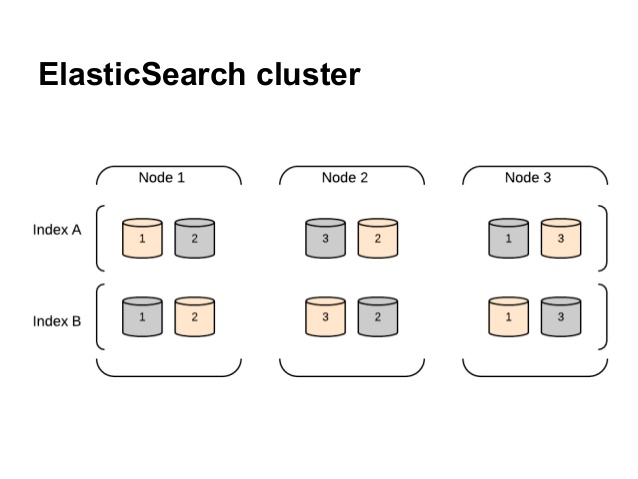
\includegraphics[width= 10cm]{ESArchitecture}
	\caption{Een cluster in Elasticsearch}
	\label{fig:ESArchitecture}
\end{figure}

\subsection{Schaalbaarheid}

Bij Elasticsearch is er sprake van horizontale schaalbaarheid \autocite{Dixit2016}. Dat wil zeggen dat een cluster opgedeeld wordt in verschillende nodes. De nodes kunnen zonder problemen op verschillende hardware functioneren. Een cluster kan dus uitgebreid worden zonder dat de complexiteit van het systeem toeneemt. Bij het toevoegen van een nieuwe node worden de shards verplaatst zodat de nodige opslagruimte minimaal blijft.

In de master thesis van \textcite{Berglund2013} wordt er een belangrijke stelling gemaakt over de schaalbaarheid van Elasticsearch. De search engine is zeer schaalbaar omdat de documents organisatorisch verdeeld zijn over verschillende nodes. Bij een specifieke zoekopdracht waarbij men zoekt op het document ID of het type zullen slechts enkele nodes moeten overlopen worden. Dat ideale scenario is echter niet altijd aan de orde. Afhankelijk van de criteria waarop men zoekt, kan het zijn dat alle nodes moeten overlopen worden. Dat is een limitatie van de schaalbaarheid van Elasticsearch. Dat probleem zou vandaag nog niet opgelost kunnen worden zonder dat er data-verlies voorkomt in de zoekresultaten. 

\subsection{Installatie}
\label{Installatie}

Elasticsearch is gratis wanneer men beslist om het zelf te hosten. De installatie verloopt zeer snel. Eerst moet men ervoor zorgen dat Java geïnstalleerd staat op het systeem. Daarna kan er een versie naar keuze van Elasticsearch gedownload worden via de website. Wanneer men het bestand uitpakt staat alles klaar om de eerste cluster op te starten. Als dat te moeilijk is kan men gebruik maken van een grafische user interface die beschikbaar is via de MSI installer package. Op de website staat stap voor stap uitgelegd hoe je de installatie kunt uitvoeren. 

Er hangen niet zoveel nadelen vast aan het zelf hosten van Elasticsearch. Men moet natuurlijk wel over voldoende ruimte beschikken op de harde schijf. Dat kan moeilijk worden wanneer men met grote hoeveelheden data werkt. Daarnaast is het belangrijk om te weten dat men zelf verantwoordelijk bent voor eventuele downtimes. Het is dus perfect mogelijk om Elasticsearch volledig gratis te gebruiken. 

Wanneer men beslist om te betalen voor de hosting bij Elasticsearch beschikt men wel over enkele voordelen. De eerder vermelde problemen in verband met ruimte op je harde schijf en downtimes zijn niet langer van toepassing. Aan de externe hosting zijn er een aantal Service Level Agreements verbonden die ervoor zorgen dat men verzekerd is van een goede kwaliteit en dat men kan rekenen op voldoende support. De kostprijs begint met 36,53 EUR per maand. Er is ook een mogelijkheid om eerst een proefversie van 14 dagen te gebruiken.

\subsection{Data importeren in Elasticsearch}

Om data te exporteren van de databank naar Elasticsearch zijn er een aantal mogelijkheden, afhankelijk van welke databank er gebruikt wordt. De eerste mogelijkheid is er één die Elasticsearch zelf aanbiedt. Daarvoor maken ze gebruik van een ander product uit de Elastic Stack\footnote{De Elastic Stack is een verzameling van open-source producten van Elastic.}: Logstash. Logstash is een ETL-tool om data te verwerken, te transformeren en uit te wisselen. Het is een product waar veel informatie en support over te vinden is. Logstash is dus een tool die veel flexibiliteit biedt maar wel een extra installatie vergt. 

Daarnaast zijn er een aantal tools die aangeboden worden door de community. Voor die tools is er in het algemeen minder support te vinden. Nog een nadeel is dat het niet altijd mogelijk is om de data naar de laatste versie van Elasticsearch te exporteren. De versies van de tools lopen namelijk in het algemeen achter op de nieuwste versie van Elasticsearch. 

Zowel Logstash als de meeste tools die worden aangeboden door de community bieden ook de functionaliteit aan om data te synchroniseren. Dat wil zeggen dat, wanneer de data verandert in de databank, die veranderingen ook doorgevoerd worden in Elasticsearch. In veel use cases zal dit veel voordelen bieden. 

\subsection{Support}

Ook support is een zeer belangrijk aspect wanneer men overweegt om met Elasticsearch te werken. Een eerste onderdeel van support is de documentatie. Hoeveel informatie kan men vinden over de werking van Elasticsearch? Volgens \textcite{Glauner2012} was die documentatie in 2012 onvoldoende. Uit het project in hoofdstuk 3 zal blijken dat deze documentatie echter zeer uitgebreid geworden is. Ook staat er een grote community achter Elasticsearch die zeer bruikbare features aanbiedt. Verder zijn er talrijke boeken te vinden (\textcite{Turner}). Deze boeken reiken van boeken waar beginners mee aan de slag kunnen tot boeken waarmee experten hun kennis verder kunnen uitbreiden.

\subsection{Gebruik van Elasticsearch}
\label{subsec:gebruikES}

Elasticsearch wordt door veel bedrijven momenteel gebruikt voor verschillende doeleinden. Die doeleinden kunnen gaan van logging tot het bestrijden van cyberaanvallen. Enkele opvallende gebruikers van Elasticsearch zijn NASA, Netflix, Github, Facebook, Cisco, Microsoft en Adobe. Deze zijn te vinden op de website van Elasticsearch.

Er kan met de REST API van Elasticsearch gecommuniceerd worden met behulp van elke web client die men prefereert. Men kan er zelf voor kiezen om deze tussenlaag over te slaan door de command line te gebruiken. Elasticsearch voorziet enkele clients die kunnen gebruikt worden in verschillende talen. Veelgebruikte talen zijn Curl, Java, C\#, Python, JavaScript, PHP, Perl en Ruby. Daarnaast biedt ook de community een uitgebreide waaier aan clients.

Elasticsearch biedt veel features zoals full text-search, completion suggesters, custom document scoring en meer. Bij full text-search geeft de gebruiker één of meerdere sleutelwoorden mee. Elasticsearch zal dan zoeken naar documents die de sleutelwoorden bevatten. Bij completion suggesters wordt opnieuw een sleutelwoord meegegeven door de gebruiker. Elasticsearch zal een lijst teruggeven met een aantal voorstellen van relevante sleutelwoorden die de gebruiker dan kan gebruiken om zijn zoektocht verder te zetten. Custom document scoring houdt in dat men zelf een functie kan meegeven die de relevantie van de zoekopdracht berekent. Variabelen die bijvoorbeeld een belangrijke rol kunnen spelen zijn de lengte van het veld, het aantal overeenkomsten en meer. Een uitgebreid aanbod aan features zorgt ervoor dat er meer kans is dat Elasticsearch aan de eisen van de use case voldoet. 

Van authorizatie is er echter geen sprake. Iedere gebruiker van Elasticsearch heeft alle rechten \autocite{Brasetvik2013}. Wanneer men bijvoorbeeld met een team van ontwikkelaars werkt moet daar rekening mee gehouden worden.

\subsection{Open source}

Elasticsearch is open source software. Dat heeft zo zijn voor- en nadelen. Iedereen kan aan de broncode om een bugfix te doen of om nieuwe features toe te voegen. Dat is zeer gunstig voor de groei van Elasticsearch. Daarnaast kan men de broncode ook aanpassen zodat er voldaan wordt aan eventuele specifieke noden van de gebruiker. \autocite{Tahir2008}

De community van Elasticsearch is groot en is zeer behulpzaam. Toch kan men daar niet altijd op vertrouwen. Wanneer men met een zeer specifiek probleem of een bug te maken heeft komt er niet altijd snel een kant en klaar antwoord. In zo'n geval staat men er alleen voor. Dat is in het algemeen zo bij open source software. Om professionele en persoonlijke hulp te krijgen zal men toch moeten betalen voor Elasticsearch.

\subsection{Alternatieven}

Er zijn heel wat alternatieven voor Elasticsearch op de markt. De meeste alternatieven bieden echter enkel functionaliteiten om data-analyses uit te voeren, om aan logging te doen of om een zoekfunctionaliteit te implementeren. Alternatieven die alle features van Elasticsearch kunnen vervangen zijn dus veel schaarser. 

\subsubsection{Algolia}

Een eerste alternatief is Algolia. Algolia is een duurder product dat zich meer op de zoekfunctionaliteit focust. Een groot verschil met Elasticsearh is de security. In tegenstelling tot Elasticsearch bestaat er in Algolia de mogelijkheid om gebruikersrechten in te voeren \autocite{Algolia}. Zo kunnen bepaalde luiken van het product afgeschermd worden voor gebruikers die daar geen toegang mogen toe hebben. Die authorizatie wordt gedaan aan de hand van API keys. Verder zal Algolia het zoekgedrag gaan analyseren zonder dat daar extra configuraties aan te pas gaan. Dat zoekgedrag kan, afhankelijk van de use case, zeer interessante informatie opleveren. Evenals Elasticsearch biedt Algolia ook logging aan. Deze functionaliteit is echter meer uitgebreid in Elasticsearch dan in Algolia. Ook de grote waaier aan aggregaties is niet aanwezig in Algolia. Data-analyses worden dus beter in Elasticsearch gedaan terwijl Algolia meer hulp kan bieden bij zoekfunctionaliteiten.

\subsubsection{Apache Solr}

Een tweede alternatief is Apache Solr. Ook deze zoekmachine werd gebouwd met Apache Lucene als basis. Apache Solr is zeer vergelijkbaar met Elasticsearch maar wordt beschouwd als een volwassen technologie terwijl Elasticsearch een jongere technologie is. Elasticsearch heeft een aantal oplossingen voor de limitaties in Solr. Die limitaties zijn ontstaan door zeer schaalbaar te willen zijn. Elasticsearch biedt meer features terwijl Apache Solr meer fout tolerant is en tegelijkertijd beter schaalt. \autocite{Solr}. Voor een eenvoudige maar robuuste zoekfunctionaliteit wordt Apache Solr aangeraden. Voor meer flexibiliteit wordt Elasticsearch aangeraden.

\subsubsection{Searchify}

Een derde alternatief is Searchify. Searchify beschikt, net als Elasticsearch, over een uitgebreid aanbod aan features. Veel van die features werden in beide zoekmachines op een andere manier geïmplementeerd maar men kan over het algemeen dezelfde resultaten bekomen. Een voorbeeld daarvan zijn de field weights in Searchify. Field weights laten de gebruiker toe om een gewicht mee te geven aan bepaalde fields in een document. Zo kan men specifiëren dat de titel van een boek een groter gewicht heeft dan de inhoud van het boek. Wanneer men nadien naar een term gaat zoeken zullen de boeken, waarvan de term in de titel zit, hoger scoren dan boeken waarvan de  term ergens in de tekst voorkomt. In Elasticsearch kan men een gelijkaardige logica bereiken met custom document scoring. Custom document scoring kwam eerder aan bod in de literatuurstudie in sectie \ref{subsec:gebruikES}. Deze feature is complexer in gebruik maar biedt meer mogelijkheden om uw zoekresultaten te beïnvloeden. Beide zoekmachines zijn beschikbaar in verschillende programmeertalen. Een aspect waar Searchify een groot voordeel bied over Elasticsearch zijn de real-time updates. Searchify is ideaal wanneer de data zeer frequent veranderd. De zoekmachine werd gebouwd om aan de noden van een moderne web site te voldoen waar de data zeer snel veranderd. Dat is het tegenovergestelde van Elasticsearch, waar data die veel veranderd ervoor kan zorgen dat men niet meer over real-time search kan spreken. Eerder in de literatuurstudie werd vermeld dat dit komt door de optimistische concurrency control. Een groot nadeel van Searchify is dat het niet gratis gebruikt kan worden. De goedkoopste module begint met 50 EUR per maand.



\section{Probleemstelling en Onderzoeksvragen}
\label{sec:onderzoeksvragen}

%% TODO:
%% Uit je probleemstelling moet duidelijk zijn dat je onderzoek een meerwaarde
%% heeft voor een concrete doelgroep (bv. een bedrijf).
%%
%% Wees zo concreet mogelijk bij het formuleren van je
%% onderzoeksvra(a)g(en). Een onderzoeksvraag is trouwens iets waar nog
%% niemand op dit moment een antwoord heeft (voor zover je kan nagaan).

De laatste dertig jaar is data zeer belangrijk geworden voor bedrijven. Ze beschikken over steeds meer data en zoeken naar nieuwe manieren om daar gebruik van te maken. Zo nemen ze belangrijke beslissingen of trekken ze conclusies aan de hand van data-analyses. Een eerste beslissing die moet gemaakt worden bij het uitvoeren van data-analyses is welke tool er zal worden gebruikt. Dat is geen gemakkelijke, maar uiterst belangrijke keuze. Er zijn veel tools beschikbaar en ze hebben allemaal andere sterktes. Omdat die keuze afhankelijk is van de use case waarvoor het zal gebruikt worden bestaat er geen universeel antwoord op dit probleem. Men kan zich enkel baseren op subjectieve meningen van anderen of op beweringen van de ontwikkelaars van de tool. Het hoofddoel van dit onderzoek is om ondersteuning te bieden bij deze keuze. In veel van die gevallen wordt Elasticsearch overwogen. Daarom worden de voor- en nadelen van de zoekmachine onderzocht. Door dit onderzoek wordt het duidelijk welke vragen men zich moet stellen bij het kiezen voor Elasticsearch. Ook de ontwikkelaars van Elasticsearch kunnen met deze voor- en nadelen rekening houden in toekomstige updates.

\section{Opzet van deze bachelorproef}
\label{sec:opzet-bachelorproef}

%% TODO: Het is gebruikelijk aan het einde van de inleiding een overzicht te
%% geven van de opbouw van de rest van de tekst. Deze sectie bevat al een aanzet
%% die je kan aanvullen/aanpassen in functie van je eigen tekst.

De rest van deze bachelorproef is als volgt opgebouwd:

In Hoofdstuk~\ref{ch:methodologie} wordt het project dat werd uitgevoerd in Elasticsearch om voor- en nadelen te introduceren, bevestigen of ontkrachten beschreven.

In Hoofdstuk~\ref{ch:conclusie}, tenslotte, wordt de conclusie gegeven en een antwoord geformuleerd op de onderzoeksvraag. Daarbij wordt ook een aanzet gegeven voor toekomstig onderzoek binnen dit domein.


%%=============================================================================
%% Methodologie
%%=============================================================================

\chapter{Methodologie}
\label{ch:methodologie}

%% TODO: Hoe ben je te werk gegaan? Verdeel je onderzoek in grote fasen, en
%% licht in elke fase toe welke stappen je gevolgd hebt. Verantwoord waarom je
%% op deze manier te werk gegaan bent. Je moet kunnen aantonen dat je de best
%% mogelijke manier toegepast hebt om een antwoord te vinden op de
%% onderzoeksvraag.

\lipsum[21-25]



%% Voeg hier je eigen hoofdstukken toe die de ``corpus'' van je bachelorproef
%% vormen. De structuur en titels hangen af van je eigen onderzoek. Je kan bv.
%% elke fase in je onderzoek in een apart hoofdstuk bespreken.

%\input{}
%\input{}
%...
%%=============================================================================
%% Conclusie
%%=============================================================================

\chapter{Conclusie}
\label{ch:conclusie}

%% TODO: Trek een duidelijke conclusie, in de vorm van een antwoord op de
%% onderzoeksvra(a)g(en). Wat was jouw bijdrage aan het onderzoeksdomein en
%% hoe biedt dit meerwaarde aan het vakgebied/doelgroep? Reflecteer kritisch
%% over het resultaat. Had je deze uitkomst verwacht? Zijn er zaken die nog
%% niet duidelijk zijn? Heeft het onderzoek geleid tot nieuwe vragen die
%% uitnodigen tot verder onderzoek?

Uit dit onderzoek komen er duidelijk meer voordelen dan nadelen. Het is echter belangrijk om voor een specifieke use case te overwegen welke eigenschappen het meest van belang zijn. Een project opzetten in Elasticsearch blijkt zeer eenvoudig te zijn. De installatie gebeurt over het algemeen in minder dan vijf minuten. Om de data te importeren bieden zowel Elasticsearch als de community verschillende mogelijkheden. Afhankelijk van de mogelijkheid die men kiest verloopt ook dat zeer vlot. Daarna kan de gebruiker meteen aan de slag zonder dat er extra configuratiewerk komt bij kijken. Het gebruik van Elasticsearch kan opgedeeld worden in verschillende luiken. Met het uitgebreid aanbod aan boeken, de gedetailleerde gids, de forums en de steeds groeiende community is er voldoende support om Elasticsearch te leren gebruiken. Om de zoekmachine aan te spreken kan men beroep doen op om het even welke web client of de command line, wat voor veel flexibiliteit zorgt. Er is sprake van een grote leercurve maar tegelijkertijd zijn er enorm veel mogelijkheden. Wanneer men voorkennis heeft van SQL Server wordt deze leercurve al voor een deel verlaagd.

Elasticsearch streeft naar real-time search maar vereenvoudigd andere zaken om dat te bereiken. Men moet zich dus afvragen hoe belangrijk real-time search is voor de use case. Ook moet men er zich van bewust zijn hoe frequent de data verandert. In een omgeving waar de data af en toe verandert is real-time search een haalbaar doel. In een omgeving waar de data zeer frequent verandert kan men soms niet meer van real-time search spreken.

Elasticsearch is ook zeer sterk in schaalbaarheid. Wanneer men werkt met data dat veel kan uitgebreid worden heeft men al een groot voordeel als men kiest voor Elasticsearch.

Join-operaties tussen verschillende indices zijn niet mogelijk. Wanneer men een relationele databank zomaar overzet zullen er ongetwijfeld tekortkomingen zijn. Men moet vooraf nadenken welke data men nodig heeft en ervoor zorgen dat die data beschikbaar is binnen eenzelfde index. Dat kan ervoor zorgen dat het importeren van de data toch niet zo vlot verloopt. Wanneer men de data-analyses slechts éénmaal wil uitvoeren is het aanmaken van de verschillende, aangepaste indices veel werk vergeleken met de waarde die men ermee creëert.

Werkt men met gevoelige data, dan kan het zijn dat Elasticsearch toch niet zo interessant is voor de use case. Er is namelijk geen sprake van authorizatie. Iedereen die het systeem gebruikt heeft alle rechten.

Men kan Elasticsearch volledig gratis gebruiken maar kan het laten hosten voor een prijs vanaf 36,53 EUR.

\subsection{Verder onderzoek}
In dit onderoek werd er onder andere kort gekeken naar enkele alternatieven voor Elasticsearch. Er werden telkens een aantal punten opgesomd waarin Elasticsearch beter scoort dan het alternatief of omgekeerd. Men zou echter veel dieper kunnen gaan in die vergelijking. In verder onderzoek zou zowel de literatuurstudie als het project kunnen herhaald worden voor de alternatieven van Elasticsearch. Aan de hand van die resultaten kan men Elasticsearch op diepgaand niveau vergelijken met de alternatieven. Op die manier kunnen er eventueel nieuwe voor- en nadelen van Elasticsearch naar boven komen die in dit onderzoek niet voorkwamen. Maar vooral wordt het makkelijker voor gebruikers om een gegronde keuze te maken van welke software ze zullen gebruiken voor hun specifieke use case.
\appendix
\chapter{Appendix}
\label{ch:appendix}

\begin{figure}
	\centering
	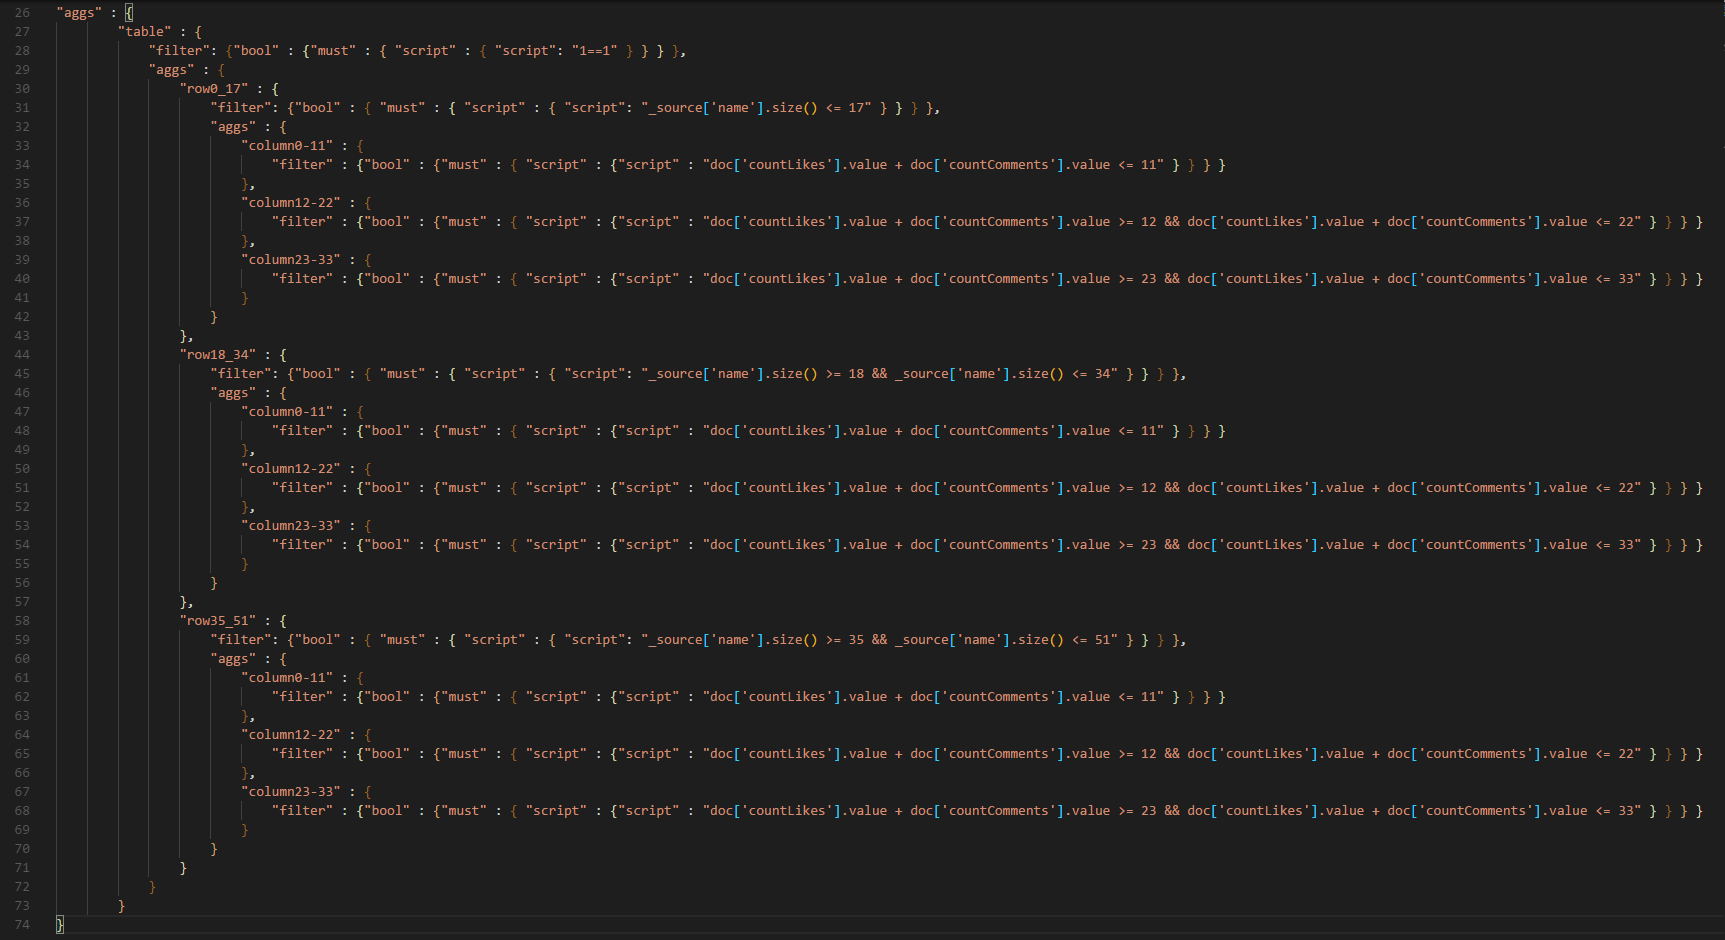
\includegraphics[width= 18cm]{script_table_wrong}
	\caption{Elasticsearch script voor het bekomen van de eerste kruistabel}
	\label{app:eersteKruistabel}
\end{figure}

\begin{figure}
	\centering
	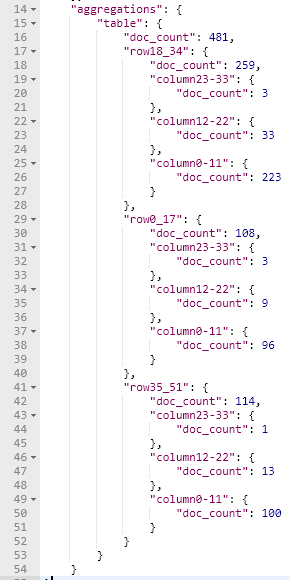
\includegraphics[width= 9cm]{script_table_wrong_result}
	\caption{Resultaat van het script voor het bekomen van de eerste kruistabel}
	\label{app:eersteKruistabelResult}
\end{figure}

\begin{figure}
	\centering
	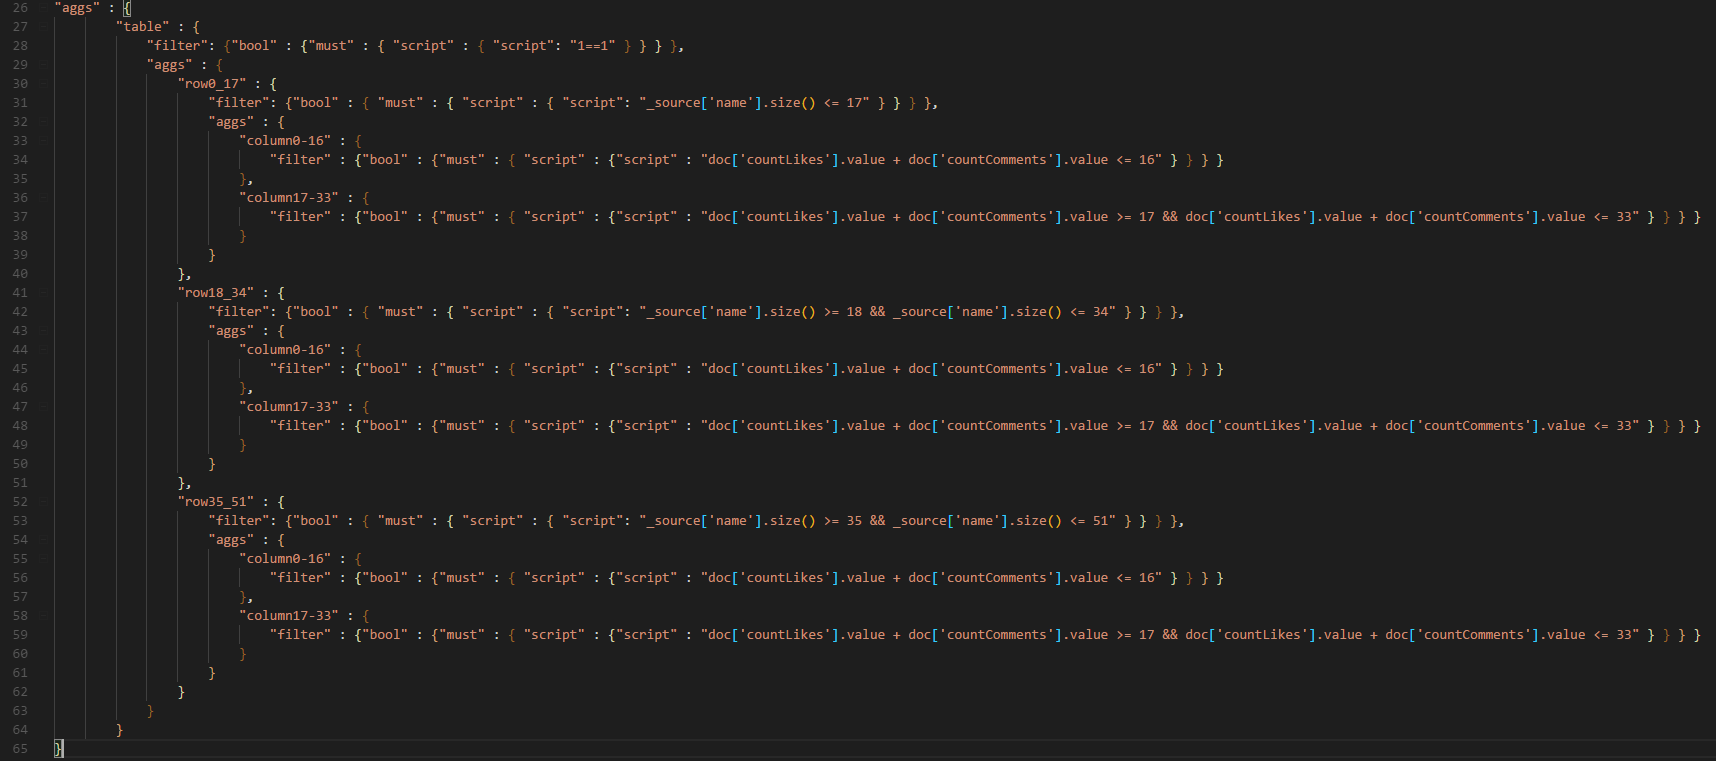
\includegraphics[width= 18cm]{script_table_correct}
	\caption{Elasticsearch script voor het bekomen van de tweede kruistabel}
	\label{app:tweedeKruistabel}
\end{figure}

\begin{figure}
	\centering
	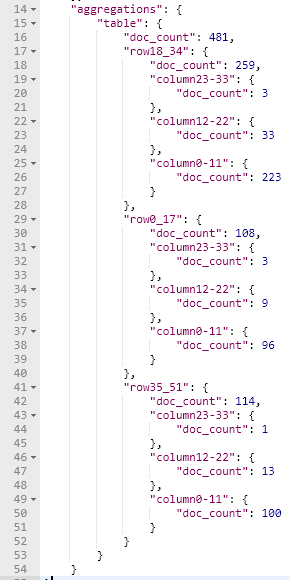
\includegraphics[width= 9cm]{script_table_wrong_result}
	\caption{Resultaat van het script voor het bekomen van de tweede kruistabel}
	\label{app:tweedeKruistabelResult}
	
\end{figure}

%%---------- Back matter ------------------------------------------------------

\printbibliography
\addcontentsline{toc}{chapter}{\textcolor{maincolor}{\IfLanguageName{dutch}{Bibliografie}{Bibliography}}}


\listoffigures
\listoftables

\end{document}
